\documentclass[PhD]{PHlab-thesis}
\PassOptionsToPackage{%
  backend=biber,   % 使用 biber 而非 bibtex
  style=numeric,   % 數字編號樣式
  sorting=none,    % 按引用次序排序
  doi=true,        % 顯示 DOI
  url=true,        % 顯示 URL
  hyperref=false   % 關閉與 hyperref 的自動整合
}{biblatex}
\usepackage{biblatex}
\addbibresource{thesis.bib}
\DeclareCiteCommand{\citeaj}
  {}% 開頭不做事
  {%
    \printnames{labelname}% 作者
    \addcomma\space
    \printfield{journaltitle}% 期刊
    \addcomma\space
    \printfield{year}% 年份
  }% 每一筆引用要做的事
  {\addsemicolon\space}% 多筆之間用分號分隔
  {}% 結尾不做事
  
\reversemarginpar        % 避免錯誤;不關心邊註方向時可保留
\setlength{\marginparwidth}{0pt}   % 邊註寬度設 0
\setlength{\marginparsep}{0pt}     % 邊註與正文的間距也設 0




\newcommand*\Department中文{資訊工程學系}
\newcommand*\Department英文{Department of Computer Science and Information Engineering}

\newcommand*\ThesisTitle中文{WebGPU 於高效能生物資訊計算:瀏覽器端 Pair-HMM Forward 演算法之優化}
\newcommand*\ThesisTitle英文{ WebGPU for High-Performance Bioinformatics Computing: Browser-Based Optimization of the Pair-HMM Forward Algorithm}

\newcommand*\Student中文{王尊緯}
\newcommand*\Student英文{Tsun-Wei Wang}

\newcommand*\Advisor中文{賀保羅}
\newcommand*\Advisor英文{Paul Horton}

%% 果有共同指導老師可以用:
%% \newcommand*\CoAdvisorA中文{}
%% \newcommand*\CoAdvisorA英文{}
%% \newcommand*\CoAdvisorB中文{}
%% \newcommand*\CoAdvisorB英文{}


\newcommand*\YearMonth英文{July, 2025}
\newcommand*\YearMonth中文{114年7月}

\pagestyle{fancy}% Use fancyhdr

\usepackage{fancyhdr}
\pagestyle{fancy}
\setlength{\headheight}{13.6pt}
\renewcommand{\chaptermark}[1]{\markboth{Chapter \thechapter.\ #1}{}}
\fancyhead{}

\fancyhead[C]{\small\MakeUppercase{\leftmark}}


\begin{document}


% ---------- Keywords ----------
\newcommand*\Keywords英文{WebGPU, Pair-Hidden Markov Model, Bioinformatics Acceleration}
\newcommand*\Keywords中文{瀏覽器 GPU 計算、Pair-Hidden Markov Model (Pair-HMM)、生物資訊加速}


% ---------- Abstract (English) ----------
\newcommand*\Abstract英文{%
As GPU acceleration gains traction in bioinformatics \citeaj{Banerjee2017,Liu2021-bib}, conventional CUDA and OpenCL workflows still require vendor-specific driver installation and remain tethered to particular hardware, limiting online teaching and front-end clinical analysis. Standardized in 2024, \textbf{WebGPU} unifies Vulkan, Direct3D~12, and Metal under a single JavaScript API \citeaj{W3C2024-webgpu}, offering three key advantages: no installation, cross-hardware portability, and on-device data residency. Using the compute-intensive Pair-Hidden Markov Model Forward (Pair-HMM Forward) algorithm \citeaj{Durbin1998} as a case study, we assess the performance and feasibility of this emerging framework.

Building on the open-source C++/CUDA implementation by Chou Yu-Chen \citeaj{Chou2024-github}, we first develop a WebGPU baseline. We then mitigate its principal bottlenecks—frequent round-trips between the CPU and GPU, and costly BindGroup reconstruction—by introducing (i) batched submission of a single \emph{CommandBuffer} and (ii) Dynamic Uniform Offsets, yielding an optimized variant termed \emph{WebGPU-Optimized}.

Benchmarks on three devices—NVIDIA RTX 2070 Super, Apple M1, and Intel UHD 620—across sequence lengths 
from $10^{2}$ to $10^{5}$ show that the optimized version attains speed-ups exceeding $100\times$ in the best case and reaches over 84 \% of CUDA's throughput, while maintaining relative log-likelihood error below $10^{-5}$ on all devices. Even without an NVIDIA GPU, our WebGPU implementation outperforms single-threaded C++ by one to two orders of magnitude.

These findings demonstrate that pure JavaScript and WGSL can execute the Pair-HMM Forward algorithm within seconds in a web browser. We contribute two browser-specific optimization strategies and provide detailed cross-hardware performance measurements, laying the groundwork for Web-native genomic analysis tools and advancing the democratization and real-time execution of bioinformatics workloads.
}



% ---------- Abstract (Chinese) ----------
\newcommand*\Abstract中文{%
隨著 GPU 加速在生物資訊領域日益普及\citeaj{Banerjee2017,Liu2021-bib},傳統 CUDA/OpenCL 工作流程仍需安裝廠商驅動程式,且受限於特定硬體,難以支援線上教學與前端臨床分析。2024 年標準化的 \textbf{WebGPU} 以單一 JavaScript API 統合 Vulkan、Direct3D~12 與 Metal\citeaj{W3C2024-webgpu},具備「免安裝」、跨硬體可攜性與本機資料駐留三大優勢。本研究以運算密集的 Pair-Hidden Markov Model Forward(Pair-HMM Forward)演算法\citeaj{Durbin1998} 為案例,評估該新框架的效能與可行性。

我們以周育晨公開的 C++/CUDA 原始碼為基準\citeaj{Chou2024-github},首先實作 WebGPU Baseline;隨後針對 CPU 與 GPU 之間頻繁往返,以及 BindGroup 重建耗時等瓶頸,依序導入「單一 \emph{CommandBuffer} 批次提交」與「Dynamic Uniform Offsets」,形成 \emph{WebGPU-Optimized}。

在 NVIDIA RTX 2070 Super、Apple M1 與 Intel UHD 620 三款裝置上,針對序列長度從 $10^{2}$ 到 $10^{5}$ 的測試顯示:優化版本在最佳情況下可獲得逾 $100\times$ 的加速,並達到 CUDA 效能的 84\% 以上;三裝置的相對 log-likelihood 誤差皆低於 $10^{-5}$。即便無 NVIDIA GPU,本方法仍較單執行緒 C++ 提供一至二個數量級的加速效果。

研究結果證實,僅憑 JavaScript 與 WGSL,即能在瀏覽器中於秒級完成 Pair-HMM Forward 計算。我們提出兩項瀏覽器端專屬優化策略,並提供跨硬體之詳細效能量測,為 Web 原生基因體分析工具奠定基礎,推動生物資訊運算的民主化與即時化。%
}






\newcommand*\Acknowledgements{%
在這裡,我想特別感謝賀保羅教授的悉心指導,以及實驗室夥伴們一路上的協助與陪伴:阮祈翰、楊祐昇、黃書堯、鄭驊軒、鄭煜醴,無論是在實驗設計還是資料處理上,大家都給了我很多寶貴的意見與支持。

也謝謝林宜靜、賴威達、王晴文、許庸袁與陳竑曄,和你們一起討論分析、Debug 程式,是這段旅程中最有趣也最有成就感的部分。

最後,感謝所有在這段期間關心、鼓勵我的師長與同學,有你們的支持,才讓這份研究能夠順利完成。 }



\newcommand*\SelectFontsize[2]{\fontsize{#1}{#1}\selectfont\mdseries#2\par}
\newcommand*\SelectFontsizeBF[2]{\fontsize{#1}{#1}\selectfont\bfseries#2\par}
\newcommand*\SignatureRule[1][6]{\rule{#1cm}{0.3mm}}
\newcommand*\AddToContents[1]{\newpage\phantomsection\addcontentsline{toc}{chapter}{#1}}

\doublespace
\pagenumbering{gobble}
\renewcommand{\thefootnote}{\fnsymbol{footnote}}


\begin{center}
\vspace{2cm}
\SelectFontsizeBF{24}{%
\University中文\Department中文\\
\學位 論文}

\vfill
\SelectFontsizeBF{24}{\ThesisTitle中文}
\ifdefined\ThesisNote中文
\SelectFontsize{22}{\textit{\ThesisNote中文}}
\fi

\vspace{5mm}
\SelectFontsizeBF{22}{\ThesisTitle英文}
\ifdefined\ThesisNote英文
\SelectFontsize{20}{\textit{\ThesisNote英文}}
\fi

\vfill

\begin{minipage}{\linewidth}
{\setlength\tabcolsep{0pt}
%
\begin{tabular}{ Wr{5em} Wl{6em} Wr{5em} wl{7em} }
研究生:   & ~~\Student中文  &      Student: & ~~\Student英文\\
指導老師: & ~~\Advisor中文  &      Advisor: & ~~\Advisor英文\\
\ifdefined\CoAdvisorA中文
共同指導: & ~~\CoAdvisorA中文 &   Co-Advisor: & ~~\CoAdvisorA英文\\
\fi
\ifdefined\CoAdvisorB中文
         & ~~\CoAdvisorB中文 &   Co-Advisor: & ~~\CoAdvisorB英文\\
\fi
\end{tabular}
}
\end{minipage}

\vfill
\SelectFontsize{18}{%
National Cheng Kung University,\\
Tainan, Taiwan, R.O.C.\\
Thesis for \ifdef\PhD{Master of Science}{Doctor of Philosophy} Degree\\
\YearMonth英文}

\vfill
\SelectFontsize{20}{中華民國\YearMonth中文}
\end{center}



\ifdefined\optCommittee
\newpage
\begin{center}
\vspace{1cm}
\SelectFontsizeBF{24}{%
\University中文\Department中文\\
\學位 論文}
\vfill
\SelectFontsizeBF{20}{\ThesisTitle中文}
\end{center}

\vfill
\SelectFontsize{20}{%
\noindent 研究生:\Student中文\\
本論文業經審查及口試合格特此證明}


\begin{center}
\SelectFontsize{18pt}{論文考試委員}
\vfill
\SignatureRule \hspace*{1cm} \SignatureRule
\vfill

\SignatureRule \hspace*{1cm} \SignatureRule
\vfill

指導教授:\SignatureRule[8]
\vfill
  所長:\SignatureRule[8]

\vfill
\SelectFontsize{18}{中華民國 \hspace{2em} 年 \hspace{2em} 月 \hspace{2em} 日}
\end{center}


\newpage
\begin{center}
\vspace{1cm}
\SelectFontsize{18}{\University英文, \Department英文}
\SelectFontsize{19}{\ifdef\PhD{Ph.D.}{Master's} Degree Thesis}

\vfill
\SelectFontsizeBF{20}{\ThesisTitle英文}
\end{center}

\vfill
\SelectFontsize{18}{Student: \Student英文}

\SelectFontsize{18}{%
A thesis submitted to the graduate division in partial fulfillment of the requirement for the degree of
\ifdef\PhD{Master of Science}{Doctor of \mbox{Philosophy}}.
}

\vfill
\begin{center}
\SelectFontsize{18}{Approved by}

\vfill
\SignatureRule \hspace*{1cm} \SignatureRule

\vfill
\SignatureRule \hspace*{1cm} \SignatureRule

\vfill
Advisor: \SignatureRule[8]

\vfill
Chairman: \SignatureRule[8]

\vfill
\SelectFontsize{18}{\YearMonth英文}
\vspace*{20pt}
\end{center}
\fi% optCommittee


\AddToContents{中文摘要}
\setcounter{page}{1}
\pagenumbering{roman}


\begin{center}
\SelectFontsizeBF{24}{\ThesisTitle中文}

\vspace{4mm}
\SelectFontsize{18}{\Student中文\footnote[1]{學生} ~ \Advisor中文\footnote[2]{指導教授}}

\vspace{5mm}
\SelectFontsize{20}{國立成功大學\Department中文}

\vspace{12mm}
\makebox[2.7cm][c]{\SelectFontsizeBF{22}{摘要}}
\end{center}

\vspace{4mm}
\SelectFontsize{16}{\Abstract中文}

\vspace{4mm}
\begin{flushleft}
\SelectFontsize{16}{\textbf{關鍵詞:} \Keywords中文}
\end{flushleft}



\AddToContents{Abstract}
\begin{center}
\SelectFontsizeBF{22}{\ThesisTitle英文}

\vspace{4mm}
\SelectFontsize{18}{\Student英文\footnote[1]{Student} ~ \Advisor英文\footnote[2]{Advisor}}

\vspace{4mm}
\SelectFontsize{16}{\Department英文, National Cheng Kung University}

\vspace{12mm}
\SelectFontsizeBF{20}{Abstract}
\end{center}

\vspace{4mm}
\SelectFontsize{14}{\Abstract英文}

\vspace{4mm}
\begin{flushleft}
\SelectFontsize{16}{\textbf{Keywords:} \Keywords英文}
\end{flushleft}



\AddToContents{誌謝}
\begin{center}\SelectFontsizeBF{24}{誌謝}\end{center}

\vspace{4mm}
\Acknowledgements



\renewcommand{\contentsname}{CONTENTS}
\AddToContents{Contents}
\tableofcontents


\AddToContents{List of Tables}
\listoftables


\AddToContents{List of Figures}
\listoffigures
% 封面頁, 口委中英文簽名單, 誌謝, 中英文摘要, 論文目錄, 圖表目錄


\renewcommand\nomgroup[1]{%
  \item[\bfseries
  \ifstrequal{#1}{A}{General}{%
  \ifstrequal{#1}{Z}{Gene/Protein Names}%
  }]}

% === A. General ===
\nomenclature[A]{HPC}{High-Performance Computing}
\nomenclature[A]{API}{Application Programming Interface}
\nomenclature[A]{BWA}{Burrows–Wheeler Aligner}
\nomenclature[A]{GATK}{Genome Analysis Toolkit}

% === B. Algorithm / Computational Model ===
\nomenclature[B]{HMM}{Hidden Markov Model}
\nomenclature[B]{SIMD}{Single Instruction Multiple Data}
\nomenclature[B]{FMA}{Fused Multiply-Add instruction}
\nomenclature[B]{SM}{Streaming Multiprocessor (CUDA core block)}
\nomenclature[B]{LUT}{Lookup Table}

% === C. GPU / WebGPU & Related Technologies ===
\nomenclature[C]{CUDA}{Compute Unified Device Architecture}
\nomenclature[C]{OpenCL}{Open Computing Language}
\nomenclature[C]{WASM}{WebAssembly}
\nomenclature[C]{WASM-SIMD}{SIMD extension of WebAssembly}
\nomenclature[C]{WGPU}{Cross-platform WebGPU API implementation}
\nomenclature[C]{ALU}{Arithmetic Logic Unit}
\nomenclature[C]{UMA}{Unified Memory Architecture}
\nomenclature[C]{DRAM}{Dynamic Random-Access Memory}
\nomenclature[C]{TFLOPS}{Tera Floating-Point Operations per Second}
\nomenclature[C]{SDK}{Software Development Kit}


\printnomenclature[5cm]

\newpage
\setcounter{page}{1}
\pagenumbering{arabic}

\chapter{Introduction}

\section{Background}
High-throughput sequencing (HTS), commonly known as next-generation sequencing (NGS), has driven an exponential growth in genomic data \cite{Mardis2017}. Such scale places unprecedented demands on computational throughput.  
The \textbf{Pair-Hidden Markov Model Forward algorithm} (Pair-HMM Forward), a core kernel for sequence alignment, genotype calling, and variant detection \cite{Durbin1998}, is among the most compute-intensive steps in modern pipelines.

State-of-the-art workflows—GATK \cite{McKenna2010}, Samtools \cite{Li2009}, and BWA-MEM2 \cite{Vasimuddin2019}—are primarily written in C++ or Python and achieve acceleration via \\ NVIDIA CUDA or OpenCL \cite{Liu2021-bib,Banerjee2017}. Besides installing drivers, SDKs, and various dependencies, users are locked to specific GPU architectures. In classrooms or resource-constrained labs, the absence of high-end GPUs—or limited cloud quotas—often forces a CPU fallback, inflating cost and turnaround time.  
Cloud services alleviate local setup but introduce account management overhead, network latency, and concerns over sensitive-data exposure.

Since WebGPU reached Chrome stable in May 2024 \cite{Chrome2024-blog}, Firefox Nightly and Edge Dev have followed with experimental support. By mapping Vulkan, Direct3D~12, and Metal to a single JavaScript API inside the browser sandbox \cite{W3C2024-webgpu}, WebGPU enables real-time parallel computation on NVIDIA, AMD, Intel, and Apple Silicon GPUs without any driver installation. This opens a new path to lowering the entry barrier for bioinformatics tools—particularly in teaching, clinical front-ends, and low-resource settings.

\section{Motivation and Objectives}
While WebGPU promises zero installation, cross-hardware portability, and on-device data residency, it was designed primarily for graphics and machine-learning inference. A dynamic-programming kernel such as Pair-HMM Forward encounters several obstacles:

\begin{itemize}
  \item \textit{API scheduling overhead} – Wavefronts must be processed sequentially; if each dispatch creates fresh command buffers and bind groups, CPU ↔ GPU round-trips accumulate rapidly.
  \item \textit{Lack of global synchronization} – Every wavefront depends on the previous one, yet WebGPU exposes only workgroup-level barriers and lacks CUDA-style kernel-return global sync \cite{W3C2024-webgpu}.
  \item \textit{Absence of dedicated special-function units (SFUs)} – Pair-HMM issues many \verb|log|/\verb|exp| calls. CUDA's SFUs finish $\log_{2}$ in four cycles \cite{NVIDIA2023-cudaguide}, whereas WebGPU must approximate via alu + lut + fma, incurring a 2–4$\times$ latency penalty.
  \item \textit{High memory-access demand} – The DP matrix resides in a read–write storage buffer; WebGPU's default path bypasses L1 cache, so frequent global reads/writes incur heavy DRAM traffic \cite{Liu2021-bib}.
\end{itemize}

These limitations leave WebGPU's suitability for bioinformatics unverified. We therefore ask: \textit{Can a browser-resident WebGPU implementation execute Pair-HMM Forward with practical performance compared with CUDA?}

Our objectives are:
\begin{enumerate}
  \item identify the dominant bottlenecks when porting Pair-HMM Forward to WebGPU;
  \item design WebGPU-specific optimizations that mitigate those bottlenecks;
  \item benchmark performance and accuracy across heterogeneous GPUs.
\end{enumerate}

\section{Methods and Key Results}
Using the open-source C++/CUDA reference by Yu-Chen Chou \cite{Chou2024-github} as baseline, we introduce two WebGPU-specific optimizations:

\begin{enumerate}
  \item \textit{Single-command-buffer batch submission} – Aggregate multiple wavefronts into one \verb|queue.submit()|, eliminating excessive API latency.
  \item \textit{Dynamic uniform offsets} – Store static parameters in a single uniform buffer and access them via dynamic offsets, omitting repeated UBO allocation and binding.
\end{enumerate}

On an NVIDIA RTX 2070 Super, across sequence lengths 100–100 000, the optimized version accelerates the baseline by 6.8–142$\times$ and attains 11–84 \% of CUDA's throughput. On Apple M1 and Intel UHD 620, it delivers 4–463$\times$ speed-ups over single-threaded C++ when sequences are $\ge1\,000$, while maintaining log-likelihood errors below $10^{-5}$.

\section{Conclusions and Contributions}
This study demonstrates that JavaScript plus WGSL can solve medium- to large-scale Pair-HMM Forward instances within seconds inside a browser sandbox. The two complementary browser-side optimizations effectively mitigate API, synchronization, and memory bottlenecks, and cross-vendor experiments on NVIDIA, Apple, and Intel GPUs confirm hardware agnosticism.  
Our findings pave the way for “open-the-browser-and-compute” genomic analysis and provide an empirical basis for future work on FP64 support and WASM-SIMD + WebGPU hybrid acceleration.





\chapter{Related Work}

\section{High-Performance Computing Requirements in Bioinformatics}

\subsection{Next-Generation Sequencing and Its Computational Challenges}
The rapid advance of next-generation sequencing (NGS) has driven genomic data volumes to grow exponentially \cite{Mardis2017}. According to Illumina, a NovaSeq X Plus equipped with a 25 B flow cell operating in dual-lane mode can produce approximately $5.2\times10^{10}$ paired-end reads ($2\times150$ bp) in a single 48-hour run—roughly $3.25\times10^{11}$ bases per hour \cite{Illumina2024-novaseqx}. Such throughput demands sequence-alignment and probabilistic computations that far exceed the capacity of traditional CPU-only architectures.

Alignment tools such as BWA \cite{LiDurbin2010} and Bowtie \cite{Langmead2009} routinely process millions to billions of reads. Although their worst-case complexity is $O(NM)$, FM-index–based seeding and extension render the average cost nearly linear, $O(L)$, in read length $L$ \cite{Ferragina2000}. To sustain these workloads, researchers increasingly employ high-performance computing (HPC) resources—especially GPUs—to meet the near-real-time requirements of modern workflows \cite{Liu2021-bib}.

\subsection{The Central Role of the Pair-HMM Forward Algorithm}
The Pair-Hidden Markov Model (Pair-HMM) Forward algorithm is fundamental to sequence alignment and genotype inference, underpinning pipelines such as GATK \cite{McKenna2010} and Samtools \cite{Li2009}. With time complexity $O(NM)$ and memory that can be reduced to $O(\max\{N,M\})$ \cite{Durbin1998,Banerjee2017}, it becomes the dominant bottleneck for long reads ($N\approx10^{4}$). Recent work shows that GPU parallelisation can shorten runtime dramatically—for example, Schmidt et al.\ \cite{Schmidt2024-gpuPairHMM} report reducing the analysis of $32\times12$ kb fragments on an NVIDIA RTX 4090 from hours to under three minutes. Nevertheless, the algorithm's performance remains highly sensitive to memory-access patterns and numerical precision, demanding hardware-aware optimisation.

\section{Conventional GPU Acceleration Frameworks: CUDA and OpenCL}

\subsection{CUDA in Bioinformatics}
NVIDIA's CUDA has become the de-facto standard for GPU computing in bioinformatics. Liu et al.\ \cite{LiuWirawan2013} introduced CUDASW++ 3.0, accelerating the Smith–Waterman algorithm by $30$–$90\times$ over a single CPU core. Schmidt et al.\ \cite{Schmidt2024-gpuPairHMM} applied CUDA to Pair-HMM Forward, achieving high throughput in large-scale genotyping pipelines. However, CUDA is confined to NVIDIA hardware and requires driver plus toolkit installation, raising the barrier for non-expert users. Furthermore, kernels often need retuning for each micro-architecture (e.g., Ampere, Hopper), hindering portability.

\subsection{OpenCL's Cross-Platform Ambition}
OpenCL aspires to hardware-agnostic GPU acceleration across NVIDIA, AMD, and Intel devices. Stone et al.\ \cite{Stone2010-opencl} demonstrated its scientific potential by accelerating molecular-dynamics simulations. Despite this promise, OpenCL is less prevalent in bioinformatics than CUDA, owing to uneven hardware support and a steeper learning curve. Klöckner et al.\ \cite{Klockner2012} observed that OpenCL's memory-management and synchronisation semantics vary widely between vendors, leading to unpredictable performance. In addition, its library ecosystem is less mature, further constraining adoption.

\subsection{Barriers and Limitations of Traditional Frameworks}
Although CUDA and OpenCL can deliver substantial speed-ups, both entail intricate setup—driver installation, SDK configuration, and dependency management—that hampers deployment in educational and clinical settings. Cloud GPUs (e.g., AWS, Google Cloud) reduce local overhead but introduce latency and data-privacy concerns \cite{Krampis2012}. Moreover, these frameworks remain tightly coupled to specific hardware and offer limited cross-platform portability, restricting their usefulness on resource-constrained devices such as laptops or embedded systems.





\section{The Emergence and Technical Characteristics of WebGPU}

\subsection{Technical Background}
On 19 December 2024, WebGPU advanced to the W3C Candidate Recommendation Snapshot stage; it has not yet reached full Recommendation status and therefore still awaits complete implementations and interoperability tests \cite{W3C2024-webgpu}. Figure~\ref{fig:webgpu-mapping} illustrates the architecture: a single JavaScript / TypeScript API translates application calls to Vulkan, Direct3D~12, or Metal back-ends, which are then dispatched to the underlying GPU. This design offers three major advantages—no driver installation, cross-platform compatibility, and browser sandbox safety \cite{Chrome2024-blog}.

WebGPU's compute pipeline is written in WGSL (WebGPU Shading Language). WGSL supports high-performance matrix operations, explicit address-space qualifiers (\verb|storage|, \verb|uniform|, \verb|workgroup|), and deterministic compilation to SPIR-V or Metal Shading Language, making it suitable for compute-intensive workloads \cite{W3C2024-webgpu}.

\begin{figure}[htbp]
    \centering
    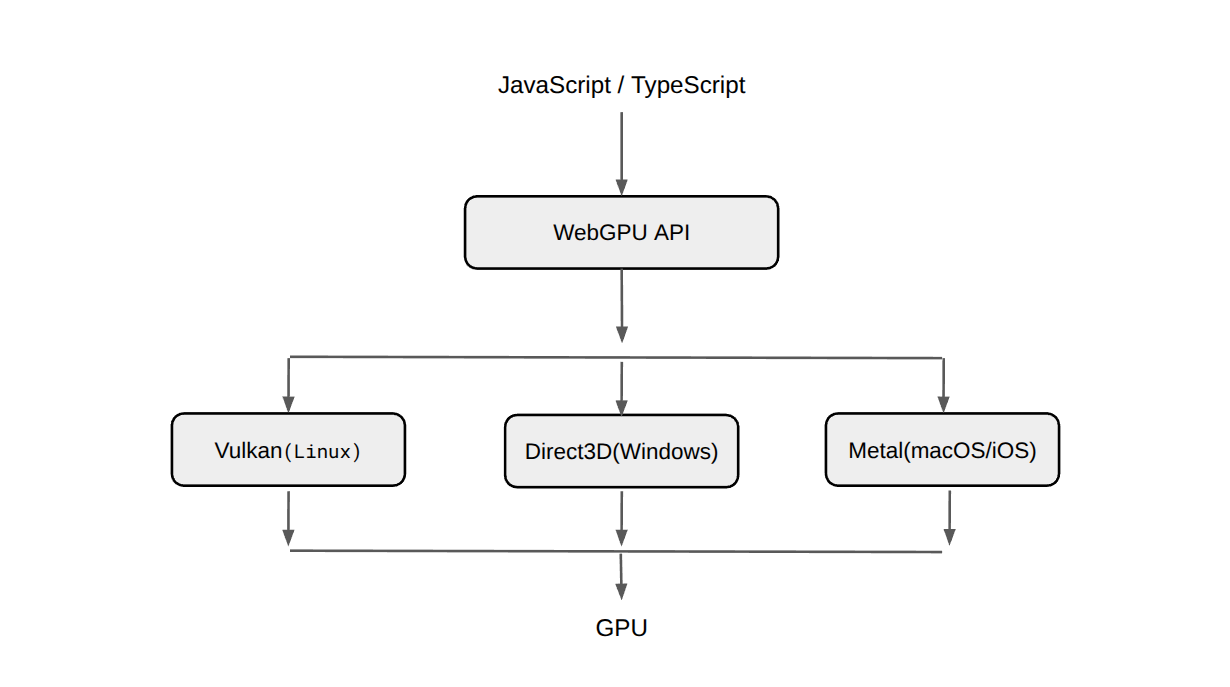
\includegraphics[width=1\linewidth]{WebGPU 架構對應示意.png}
    \caption{Mapping between the WebGPU API and native back ends}
    \label{fig:webgpu-mapping}
\end{figure}

JavaScript/TypeScript invokes WebGPU through a unified interface. The browser selects Vulkan (Linux), Direct3D~12 (Windows), or Metal (macOS/iOS) as the actual back end and submits commands to the GPU.

\subsection{High-Performance Computing Potential of WebGPU}
Early evidence from graphics and machine-learning workloads signals \\ WebGPU's competitiveness. MDN Web Docs reports in-browser rendering throughput comparable to native Vulkan \cite{MDN2025-webgpuapi}; TensorFlow.js accelerates neural-network training via its WebGPU back-end \cite{TensorFlowJS2024-webgpu}. The Google Chrome Team further shows that Transformers.js running BERT-base on an NVIDIA RTX~4060 Laptop is about $32.51\times$ faster in WebGPU mode than in WebAssembly \cite{ChromeTeam2024-recap}. These results indicate that WebGPU's execution model can leverage GPU parallelism efficiently.  
Nevertheless, bioinformatics imposes stricter requirements on numerical precision and memory efficiency. WebGPU trades some low-level control for portability, which differentiates its compute shaders from those of conventional GPU frameworks.

\subsection{Challenges and Limitations of WebGPU}
Despite its cross-platform appeal, WebGPU still faces several hurdles in high-intensity computing:

\begin{itemize}
  \item \textbf{API latency.} Each \verb|queue.submit()| or \verb|setBindGroup()| call crosses multiple layers (V8 → Blink → Dawn → driver), adding 5–15 µs of overhead \cite{ChromeTeam2024-recap}. Wavefront algorithms that dispatch hundreds of kernels per frame therefore suffer significant CPU–GPU round-trip cost.
  \item \textbf{Limited synchronisation.} WebGPU exposes only \verb|workgroupBarrier| and lacks any cross-workgroup global-synchronisation primitive \cite{W3C2024-webgpu}, complicating algorithms that require fine-grained coordination.
  \item \textbf{Restricted math support.} WGSL omits transcendental functions such as \verb|log| and \verb|exp|; these must be emulated in software or via vendor-specific SFUs, incurring additional latency. Double-precision (\texttt{f64}) is only optionally supported and remains less mature than in CUDA \cite{Jones2023-toji}.
  \item \textbf{Memory constraints.} Running inside the browser sandbox limits buffer sizes and excludes direct host-pinned memory, which becomes critical for the memory-bound wavefront updates in Pair-HMM Forward.
\end{itemize}

\section{Initial Explorations of WebGPU in Bioinformatics}
Direct WebGPU applications in bioinformatics remain scarce, yet related browser technologies provide useful precedents. Ghosh \emph{et al}. employed WebGL to create Web3DMol, proving that in-browser molecular visualisation is feasible \cite{Ghosh2018}. Jones argues that pairing WASM-SIMD with WebGPU could further accelerate sequence analysis \cite{Jones2023-toji}.  
Other compute-intensive domains offer additional insight. TensorFlow.js leverages WebGPU for high-throughput matrix operations \cite{TensorFlowJS2024-webgpu}; its buffer-reuse scheme and tiled GEMM kernels inspire our memory-layout decisions for Pair-HMM Forward. However, existing studies focus mainly on visualisation or inference tasks; implementations of demanding dynamic-programming algorithms such as Pair-HMM Forward remain unexplored. Although Schmidt \emph{et al}. provide a CUDA baseline, browser-specific optimisations have not yet been investigated \cite{Schmidt2024-gpuPairHMM}.

\section{Research Gap and Positioning of This Work}
The literature reveals three outstanding gaps:

\begin{enumerate}
  \item Lack of systematic verification of WebGPU's performance and feasibility for compute-heavy bioinformatics kernels such as Pair-HMM Forward.
  \item Absence of browser-specific optimisation strategies that target \\GPU-compute bottlenecks—namely CPU–GPU round-trips and BindGroup reconstruction. Each \verb|setBindGroup()| traverses multiple layers (V8 → Blink → Dawn → driver) and incurs ≈ 5–15 µs of latency \cite{Chrome2024-blog}, which is significant for wavefront algorithms.
  \item Insufficient evaluations across heterogeneous GPUs (NVIDIA, Apple, Intel) to gauge WebGPU's portability. Mainstream tools like GATK require CUDA and are thus tied to NVIDIA drivers, limiting use in classrooms or low-resource environments; cloud solutions raise latency and privacy concerns \cite{Krampis2012}.
\end{enumerate}

By porting Yu-Chen Chou's CUDA implementation to WebGPU, this work proposes two browser-side optimisations—\emph{single CommandBuffer batch submission} and \emph{Dynamic Uniform Offsets}—and validates their effect on performance and accuracy across multiple hardware platforms, narrowing the research gap and laying the groundwork for driver-free, cross-hardware, on-device genomic analysis tools.






\chapter{Methods}
\section{Synthetic Dataset Generation}\label{sec:dataset}
To evaluate the performance of the proposed GPU-accelerated Pair-HMM, we
dynamically generate four deterministic test sets of length
$100$, $1\,000$, $10\,000$, and $100\,000$~bp immediately before each run.
For every length~$L$, the host CPU first constructs an
$L\times4$ read-probability matrix whose nucleotide probabilities
(A, C, G, T) are all $0.25$.
It then creates a reference sequence of identical length composed entirely
of the nucleotide “A”.
Both the read profile and the reference sequence are copied to the GPU,
where the forward algorithm is executed.
By eliminating stochastic variation in the input, we can focus on how
different parallelisation strategies scale in computational and memory
efficiency as sequence length increases.

\paragraph{Provenance of the generator}%
The entire dataset-generation procedure—including the pseudo-random
probability initialiser, transition matrix, and emission constants—is
ported \emph{verbatim} from the open-source C++/CUDA reference
implementation released by Yu-Chen~Chou \cite{Chou2024-github}.
No additional code was written for dataset preparation, ensuring that our
WebGPU kernels and the CUDA baseline process identical inputs and are thus
directly comparable.

\section{Mathematical Model}
This study adopts a Pair-HMM combined with a sequence profile, following
the formulation in \cite{Durbin1998}.

Hidden states are Match (\textit{M}), Insert (\textit{I}), and Delete
(\textit{D}) over the alphabet $\{A,C,G,T,-\}$.

The read sequence is represented by a probability matrix
\[
P=[p_{i,a}],\qquad
1\le i\le m,\;
a\in\{A,C,G,T\},\;
\sum_{a}p_{i,a}=1,
\]
which gives the probability that position~$i$ of the read is character~$a$
\cite{Chou2024-github}.

The reference sequence is a fixed string $h_{1},\dots,h_{n}$.

Transition probabilities are denoted
\[
t_{XY},\qquad X,Y\in\{M,I,D\},
\]
and the base-emission matrix $\varepsilon_{X}(x,y)$ adopts the same
settings as the reference implementation \cite{Durbin1998}.

For the \emph{Match} and \emph{Insert} states, the emission probability at
alignment cell~$(i,j)$ is a probability-weighted average of the read-base
distribution at position~$i$ and the corresponding base-emission
coefficients.
The \emph{Delete} state always emits a gap, so its emission probability is~1.

\section{Pair-HMM Forward Algorithm}
The forward recursion advances along anti-diagonals (wavefronts) of the
dynamic-programming matrix, as illustrated in
Figure~\ref{fig:pairhmm-wavefront}.
Each wavefront can proceed only after the previous one completes; without
device-side global synchronisation, this dependency constitutes a major
GPU bottleneck \cite{Chou2024-github}.

\begin{enumerate}
  \item \textbf{Initialisation}
    \[
      M_{0,j}=I_{0,j}=0,\qquad
      D_{0,j}=\frac{1}{n}\quad (j>0).
    \]
  \item \textbf{Recursion} \cite{Durbin1998}
    \[
      M_{i,j}=e^{M}_{i,j}\bigl(
        t_{MM}M_{i-1,j-1}+t_{IM}I_{i-1,j-1}+t_{DM}D_{i-1,j-1}\bigr),
    \]
    \[
      I_{i,j}=e^{I}_{i,j}\bigl(
        t_{MI}M_{i-1,j}+t_{II}I_{i-1,j}\bigr),
    \]
    \[
      D_{i,j}=t_{MD}M_{i,j-1}+t_{DD}D_{i,j-1}.
    \]
  \item \textbf{Termination}
    \[
      P=\sum_{j=1}^{n}\bigl(M_{m,j}+I_{m,j}\bigr).
    \]
  \item \textbf{Complexity} The overall time complexity is
    $\mathcal{O}(nm)$, while memory usage can be reduced to
    $\mathcal{O}(\max\{n,m\})$ via two-row buffering.
\end{enumerate}

\begin{figure}[htbp]
  \centering
  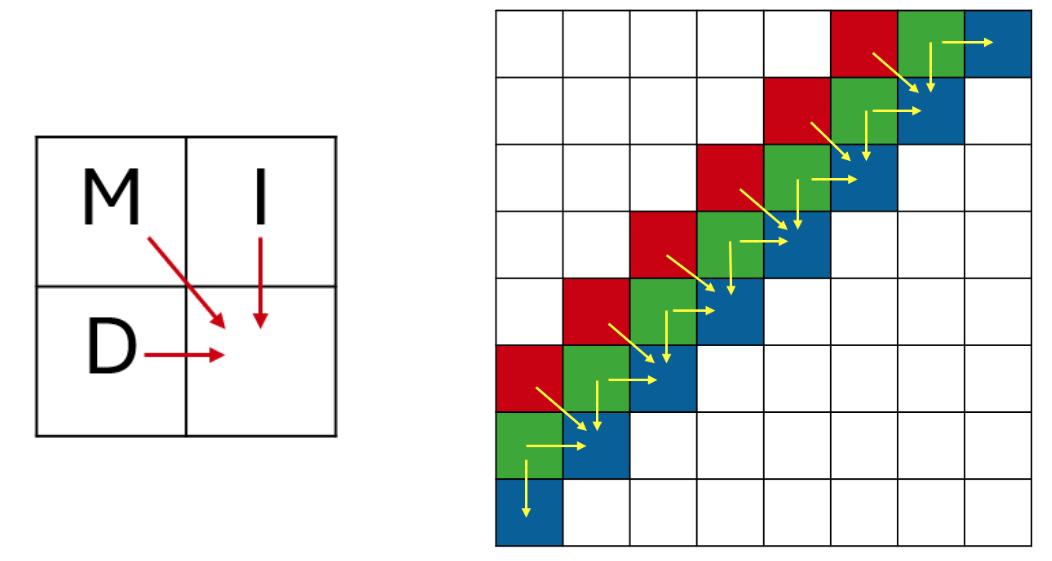
\includegraphics[width=1\linewidth]
    {Pair-HMM Forward 的計算沿反對角線 .png}
  \caption{Wavefront computation in the Pair-HMM Forward algorithm}
  \label{fig:pairhmm-wavefront}
\end{figure}

\section{System Design and Implementation}
\subsection{C++/CUDA Version}
Building on prior work showing that CUDA efficiently implements Pair-HMM via anti-diagonal parallelisation \cite{Banerjee2017,Schmidt2024-gpuPairHMM}, we adopted and refactored the open-source C++/CUDA code by Yu-Chen Chou \cite{Chou2024-github}. All double-precision (\texttt{double}) variables were converted to single precision (\texttt{float}) so the CUDA results serve as an upper-bound performance ceiling directly comparable with our WebGPU implementation. Because WebGPU currently guarantees only \texttt{f32} arithmetic \cite{W3C2024-webgpu}, retaining \texttt{f64} on CUDA would obscure cross-platform comparisons. After conversion, the maximum relative error at length $N=10^{5}$ was merely $2.18\times10^{-1}\%$, satisfying the accuracy threshold for subsequent validation.

We preserve the “one kernel per anti-diagonal” design: each of the $2N$ wavefronts launches a kernel, and a \texttt{cudaDeviceSynchronize()} between adjacent kernels acts as a GPU-wide barrier \cite{NVIDIA2023-cudaguide}. This maps the DP dependencies to device execution straightforwardly.

Global synchronisation alone cannot hide memory latency. Inside each block we therefore keep a fine-grained \texttt{\_\_syncthreads()} so that every warp shares cached values from the previous row before advancing. For the three DP arrays $M$, $I$, and $D$, we employ a host-side $4$-row pointer rotation: four $(n+1)$-length buffers are allocated once, and the host loop rotates pointers to realise the $\textit{prev}\!\rightarrow\!\textit{curr}\!\rightarrow\!\textit{new}$ shift \cite{LiuWirawan2013}. Treating CUDA pointers as ordinary C pointers avoids reallocations and \texttt{memcpy} overhead, maximising PCIe/NVLink bandwidth.

This layout also paves the way for the WebGPU port: once inside the browser we lose mutable pointers and must replace them with either BindGroup reconstruction or Dynamic Uniform Offsets \cite{Chrome2024-blog}.



\subsection{WebGPU Baseline}

\subsubsection{From CUDA “multiple kernels” to WebGPU “multiple dispatches”}
Pair-HMM Forward advances along anti-diagonals; each wavefront must finish before the next can begin \cite{Durbin1998}. The straightforward CUDA strategy is a host-side loop that launches successive kernels with a \texttt{cudaDeviceSynchronize()} between them, as in earlier studies \cite{Banerjee2017,Schmidt2024-gpuPairHMM}. Figure~\ref{fig:global-sync-diff} shows that this barrier stays entirely on the GPU.

By contrast, WebGPU lacks a device-side global barrier; synchronisation returns to JavaScript and issues a new \texttt{dispatch} \cite{W3C2024-webgpu}. For length $N$, this triggers $2N$ CPU$\leftrightarrow$GPU round-trips \cite{Chrome2024-blog}, the Baseline’s first major bottleneck.

\begin{figure}[htbp]
    \centering
    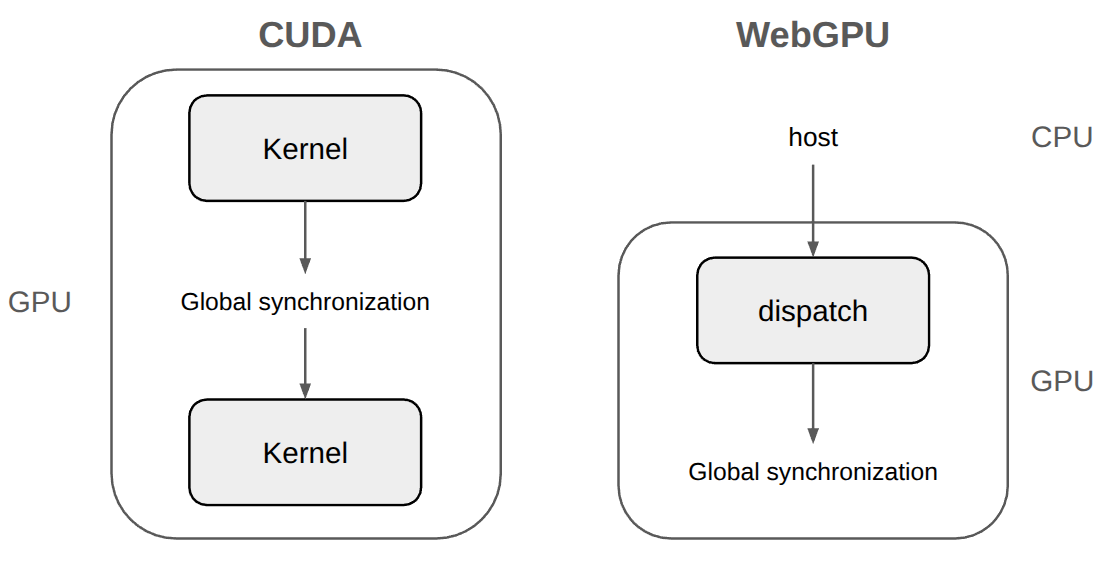
\includegraphics[width=1\linewidth]{4. 全域同步差異圖.png}
    \caption{Comparison of global synchronisation in CUDA and WebGPU}
    \label{fig:global-sync-diff}
\end{figure}

After the host calls \texttt{queue.submit()} for the current wavefront, it awaits \texttt{device.queue.onSubmittedWorkDone()} before updating uniforms and submitting the next dispatch. For $N=10^{5}$ this yields roughly $200\,000$ \(\texttt{submit}\!\rightarrow\!\texttt{await}\) cycles whose latency surfaces on the JavaScript thread.

\subsubsection{Pointer rotation versus the immutability of BindGroups}
CUDA needs only to swap three \texttt{float*} pointers between wavefronts, rotating the roles $\textit{prev}\!\rightarrow\!\textit{curr}\!\rightarrow\!\textit{new}$ without reallocating resources \cite{NVIDIA2023-cudaguide}.

In WebGPU, however, each binding slot is immutable once the BindGroup is created. To let the next wavefront read a different DP buffer, the host must call \texttt{device.createBindGroup()} again. This path crosses V8, Blink, Dawn, and the driver, adding $5$–$15$\,\textmu s per call \cite{Chrome2024-blog}, as illustrated in Figure~\ref{fig:webgpu-ipc-validation}.

\begin{figure}[htbp]
    \centering
    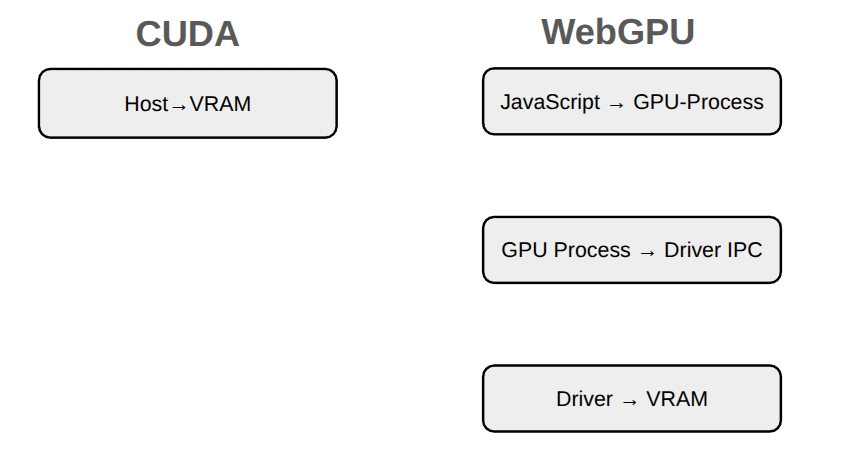
\includegraphics[width=1\linewidth]{3. WebGPU 多層 IPC/驗證路徑.png}
    \caption{Multi-layer IPC/validation path for binding a WebGPU storage buffer}
    \label{fig:webgpu-ipc-validation}
\end{figure}

\subsubsection{Performance profile of the Baseline}
On an NVIDIA RTX 2070 Super the Baseline takes about $466$ s when $N=100\,000$, nearly two orders of magnitude slower than the CUDA version on the same hardware—consistent with the overhead sources analysed above \cite{Chrome2024-blog}. Profiling attributes the delay chiefly to the $2N$ synchronisations and $2N$ BindGroup creations, motivating the optimisation strategies introduced next.





\subsection{Optimized WebGPU Version}

To remove the Baseline’s two dominant bottlenecks—
\begin{enumerate}
  \item frequent host synchronisations
  \item repeated BindGroup constructions
\end{enumerate}
—we introduce two browser-side optimisations: \emph{single-CommandBuffer batch submission} and \emph{Dynamic Uniform Offsets}. Below we first recap WebGPU’s command-recording model \cite{W3C2024-webgpu} and then detail each optimisation’s rationale, implementation, and impact.

\subsubsection{Single-CommandBuffer Batch Submission — Reducing CPU–GPU Round-Trips}
Figure~\ref{fig:scb-batch-workflow} illustrates the workflow. All $2N$ \texttt{dispatchWorkgroups} calls are recorded into one \texttt{CommandBuffer}. A single \texttt{queue.submit()} then sends the entire stream to the GPU, eliminating \(>\!99\,\%\) of IPC latency \cite{Chrome2024-blog}.

\textit{CommandEncoder and the command stream.}  
A WebGPU \texttt{CommandEncoder} records \texttt{beginComputePass}, \texttt{dispatchWorkgroups}, \texttt{copyBufferToBuffer}, \texttt{end}, and related calls. Executing \texttt{encoder.finish()} produces a \\ \texttt{GPUCommandBuffer}, which \texttt{device.queue.submit([commandBuffer])} dispatches to the GPU; the GPU then executes the complete stream without further CPU intervention \cite{W3C2024-webgpu}.

\textit{Pain points of many small submissions.}  
The Baseline issues a host-side loop that (i) rebuilds an encoder, (ii) submits, (iii) awaits completion, and then (iv) repeats—\(2N\) times for a sequence of length \(N\) \cite{Chrome2024-blog}. Each wait triggers CPU–GPU IPC and forces the JavaScript thread to oscillate between idle and active states.

\textit{Advantages of a single monolithic stream.}  
We keep the per-wavefront logic but confine it to command-recording time; the final \texttt{submit} occurs once. Driver validation and scheduling overhead collapse to a single event, and back-to-back \texttt{dispatch}/\texttt{copy} commands improve DRAM burst utilisation. Compressing \(2N\) IPC events into one markedly shortens runtime.

\begin{figure}[htbp]
  \centering
  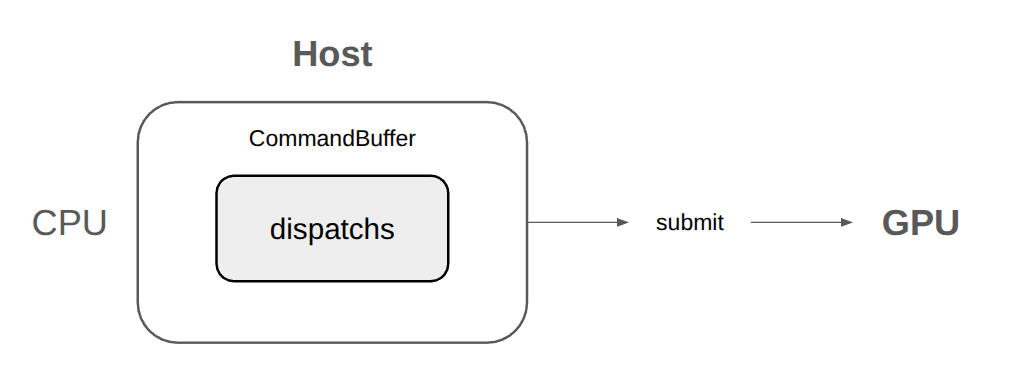
\includegraphics[width=0.9\linewidth]{1. 單一 CommandBuffer 示意圖.png}
  \caption{Single-CommandBuffer batch-submission workflow}
  \label{fig:scb-batch-workflow}
\end{figure}

\subsubsection{Dynamic Uniform Offsets — Cutting Constant-Update Overhead}
Per-wavefront constants \texttt{(len, diag, numGroups)} are packed sequentially into a single uniform buffer, each block aligned to 256 bytes (Figure~\ref{fig:dynamic-offset-layout}). WebGPU permits a 256-byte-aligned dynamic offset in \texttt{setBindGroup()} \cite{W3C2024-webgpu}. At dispatch time the correct block is selected via this offset, so buffer objects remain unchanged even though \texttt{createBindGroup()} is still invoked. In practice the validation cost per call drops by roughly 20–30 \% \cite{Chrome2024-blog}.

\begin{figure}[htbp]
  \centering
  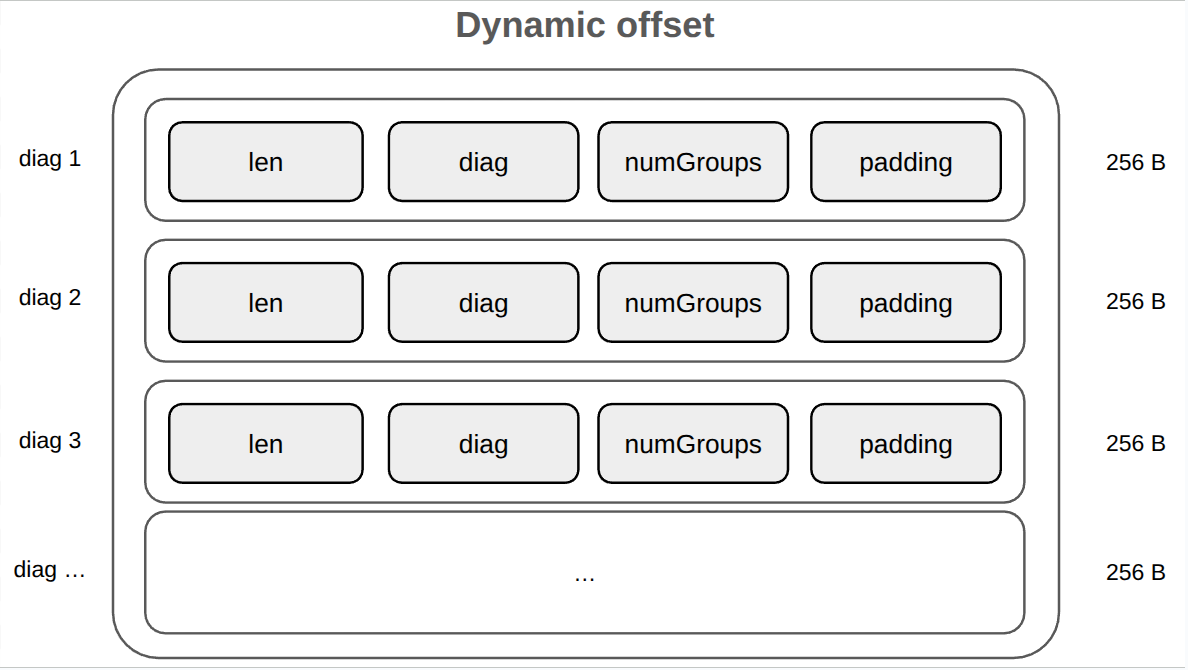
\includegraphics[width=1\linewidth]{2. Dynamic Offset 佈局圖.png}
  \caption{Data layout for Dynamic Uniform Offsets}
  \label{fig:dynamic-offset-layout}
\end{figure}
\newpage
%------------------------------------------------
\section{Summary}

Enabling both browser-side optimisations yields the results in Table~\ref{tab:opt_performance}. On an RTX 2070 Super, total runtime falls from $466$ s to $74$ s—an 84 \% reduction (our measurements, 2025).

\begin{table}[h]
  \centering
  \setlength{\tabcolsep}{6pt}
  \renewcommand{\arraystretch}{1.35}
  \small
  \begin{tabularx}{\textwidth}{|X|c|c|c|}
    \hline
    Metric & Baseline & Optimized & Reduction \\
    \hline
    CPU–GPU round-trips & $2N$ & $1$ & $99\,\%\!\downarrow$ \\
    BindGroup entries    & $2N \times \ge 10$ & $2N \times 7$ & $30\,\%\!\downarrow$ \\
    \hline
  \end{tabularx}
  \caption{Performance gains obtained by the two browser-side optimisations}
  \label{tab:opt_performance}
\end{table}

With the optimisations applied, the WebGPU implementation trails CUDA by only 19 \% for a \(100\,000\)-base sequence yet remains nearly three orders of magnitude faster than single-threaded CPU execution, demonstrating that near-native GPU performance is achievable entirely within the browser sandbox.





	
\chapter{Results}

\section{Experimental Environment}

To ensure reproducibility, all WebGPU tests were conducted in Chrome \\ 135.0.7049.95 \cite{Chrome2024-blog}. The Apple M1 and Intel UHD 620 platforms were upgraded to the same browser build; corresponding operating-system versions are listed in Table~\ref{tab:exp_env}.

Table~\ref{tab:exp_env} summarises the hardware configurations and software stacks \cite{NVIDIA2019-rtx2070,Apple2020-m1,Intel2018-uhd620} that serve as baselines for later experiments.

\begin{table}[htbp]
  \centering
  \caption{Experimental environment}
  \label{tab:exp_env}
  \setlength{\tabcolsep}{8pt}
  \renewcommand{\arraystretch}{1.4}
  \small
  \begin{tabularx}{\textwidth}{@{}lX X X X@{}}
    \toprule
    Category & Parameter & RTX 2070 Super & Apple M1 GPU & Intel UHD 620 \\
    \midrule
    CPU      & Model                 & Ryzen 7 3700X          & Apple M1 (4P+4E)   & Core i5-8265U \\
    GPU      & SM / FP32 Peak        & 40 SM – 9.1 TFLOPS     & 8 cores – 2.6 TFLOPS & 24 EU – 0.35 TFLOPS \\
    OS       & Version               & Ubuntu 24.04.2 LTS     & macOS 14.4          & Windows 11 22H2 \\
    Browser  & Version               & Chrome 135.0.7049.95   & Chrome 135.0.7049.95 & Chrome 135.0.7049.95 \\
    CUDA drv & Toolkit / Driver      & 12.0 / 550.54          & —                   & — \\
    \bottomrule
  \end{tabularx}
\end{table}


\section{Performance Data}

\subsection{RTX 2070 Super: Runtime and Relative Ratios}
Wall-clock time $T(N)$ denotes the elapsed interval from host invocation to
result retrieval, including GPU-memory allocation and the
\texttt{queue.submit()} call.

Table~\ref{tab:rtx_performance} reports the measured runtimes of four
implementations—CPU, CUDA, WebGPU-Baseline (Init), and WebGPU-Optimized
(Opt.)—for each sequence length $N$, together with the time ratios
\[
  R_{X/\mathrm{Opt}}(N)=\frac{T_{X}(N)}{T_{\mathrm{Opt}}(N)},
\]
where values $>1$ indicate that WebGPU-Optimized is faster than
$X$, and values $<1$ indicate that it is slower.

\begin{table}[ht]
  \centering
  \caption{Wall-clock runtime and relative ratios on the RTX 2070 Super
           (\textbf{CPU/Opt.} = $T_{\text{CPU}}/T_{\text{Opt}}$;
            \textbf{CUDA/Opt.} = $T_{\text{CUDA}}/T_{\text{Opt}}$).}
  \label{tab:rtx_performance}
  \renewcommand{\arraystretch}{2}
  \setlength{\tabcolsep}{4pt}
  \small
  \begin{tabular}{|c|c|c|c|c|c|c|}
    \hline
    $N$ & CPU (s) & CUDA (s) & WebGPU-Baseline (s) & WebGPU-Optimized (s) & CPU/Opt. & CUDA/Opt. \\
    \hline
    $10^{2}$ & 0.00330   & 0.00229  & 0.135 & 0.020 & 0.165 & 0.115 \\
    $10^{3}$ & 0.327     & 0.0208   & 0.602 & 0.043 & 7.60  & 0.484 \\
    $10^{4}$ & 32.80     & 0.1908   & 21.83 & 0.346 & 94.8  & 0.551 \\
    $10^{5}$ & 3\,275.6  & 2.7696   & 466.8 & 3.299 & 993   & 0.840 \\
    \hline
  \end{tabular}
\end{table}




\begin{figure}[htbp]
  \centering
  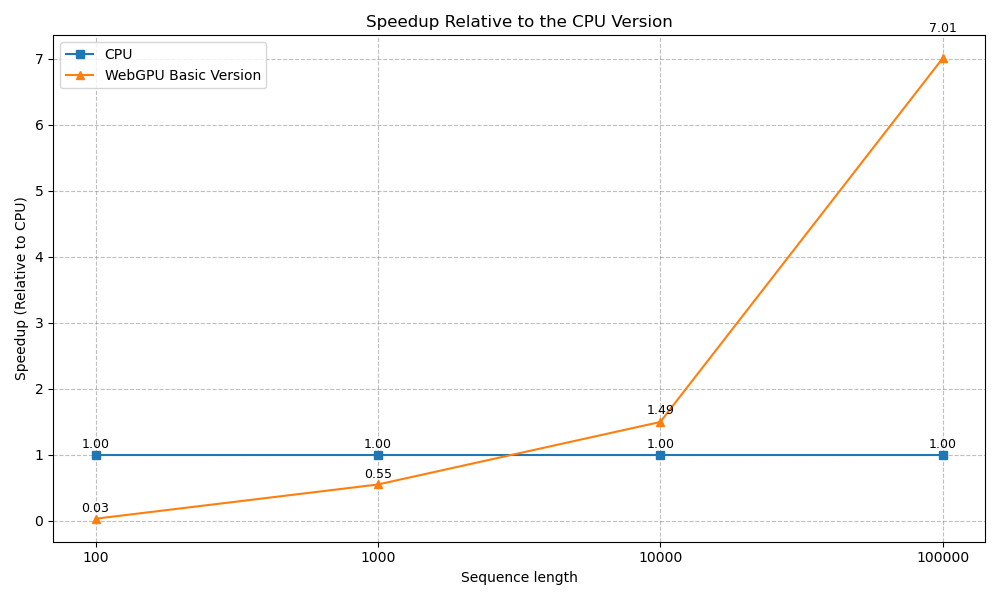
\includegraphics[width=1\linewidth]{2070s-1.png}
  \caption{Speed-up of WebGPU-Baseline over CPU on the RTX 2070 Super}
  \label{fig:2070s-wgpu-baseline}
\end{figure}

\begin{figure}[htbp]
  \centering
  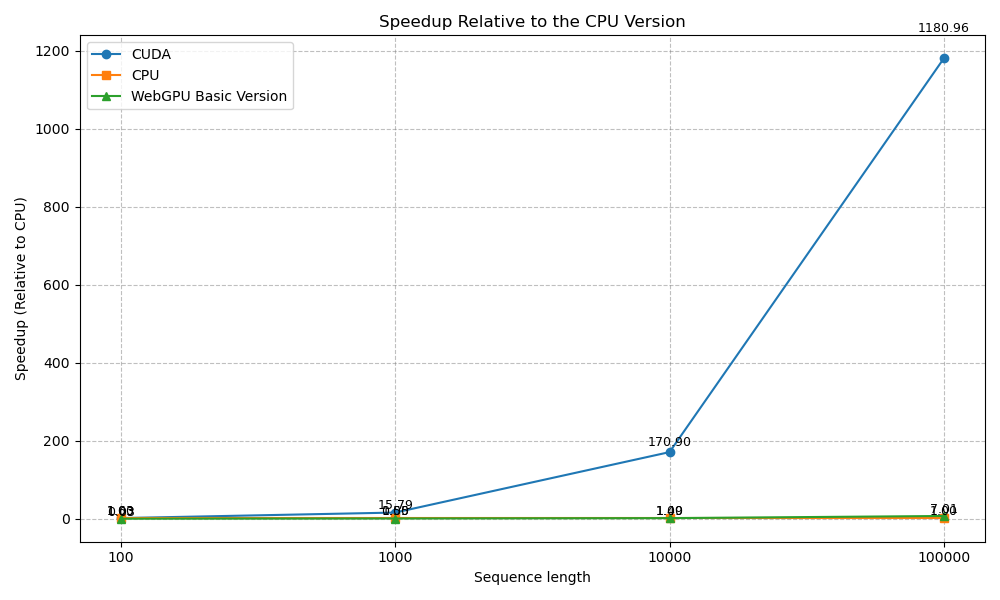
\includegraphics[width=1\linewidth]{2070s-3.png}
  \caption{Speed-up comparison of CUDA and WebGPU-Baseline (CPU = 1.0)}
  \label{fig:2070s-cuda-vs-baseline}
\end{figure}

\begin{figure}[htbp]
  \centering
  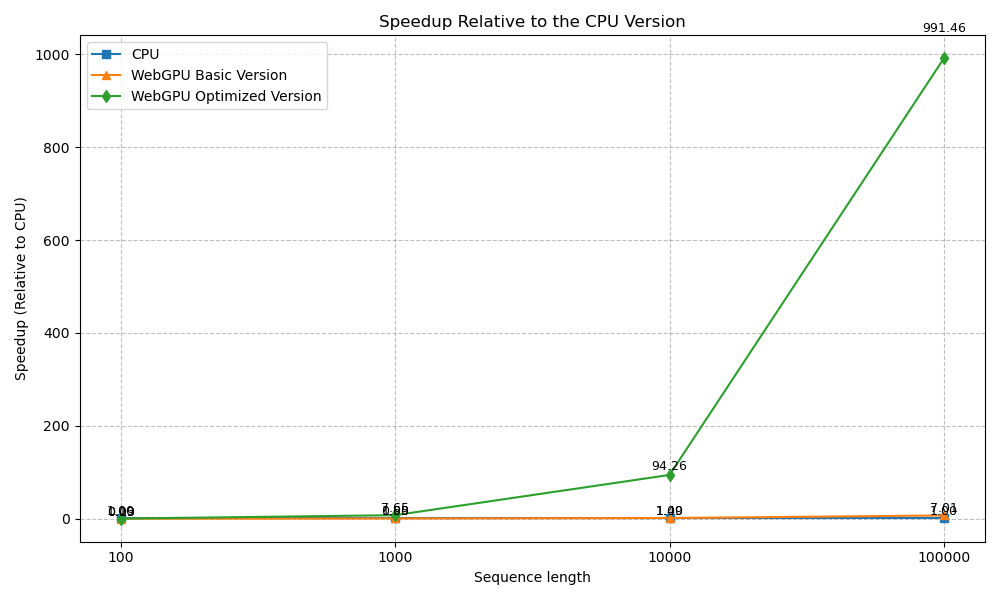
\includegraphics[width=1\linewidth]{2070s-2.png}
  \caption{Speed-up of WebGPU-Optimized versus Baseline on the RTX 2070 Super}
  \label{fig:2070s-optimized-vs-baseline}
\end{figure}

\begin{figure}[htbp]
  \centering
  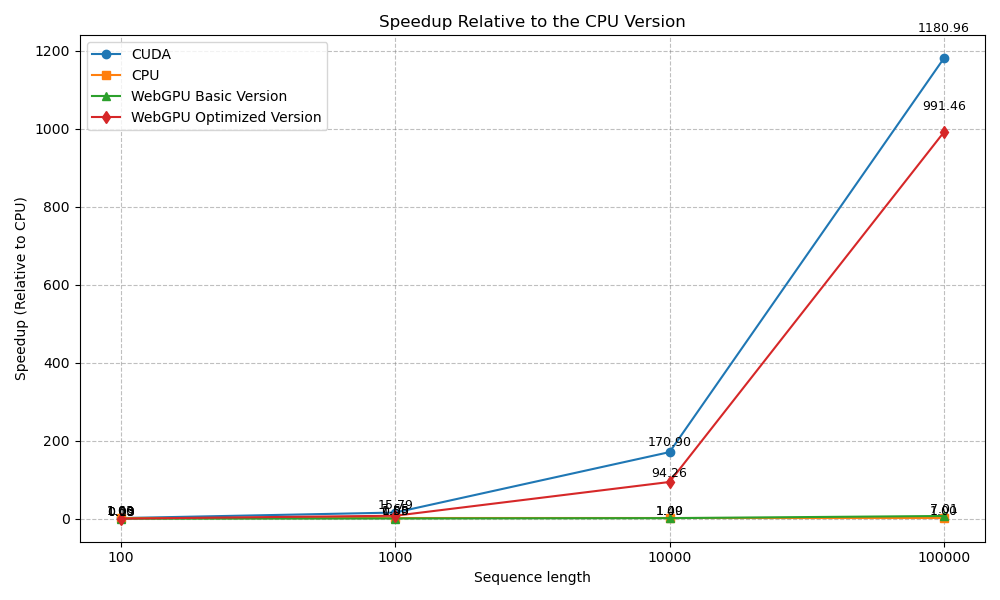
\includegraphics[width=1\linewidth]{2070s-4.png}
  \caption{Overall comparison of the four versions on the RTX 2070 Super}
  \label{fig:2070s-overall-4versions}
\end{figure}

\newpage


\subsection{Apple M1 and Intel UHD 620: Cross-Platform Results}
Because these integrated GPUs lack CUDA support\cite{Apple2020-m1,Intel2018-uhd620}, we report WebGPU-Optimized acceleration relative to CPU:
\[
S_{\text{Opt}\leftarrow\text{CPU}}(N)=\frac{T_{\text{CPU}}(N)}{T_{\text{Opt}}(N)} .
\]

\begin{table}[h]
  \centering
  \renewcommand{\arraystretch}{1.9}
  \setlength{\tabcolsep}{4pt}
  \small
  \begin{tabularx}{\textwidth}{|c|
    >{\centering\arraybackslash}X|
    >{\centering\arraybackslash}X|
    >{\centering\arraybackslash}X|
    >{\centering\arraybackslash}X|
    >{\centering\arraybackslash}X|
    >{\centering\arraybackslash}X|}
    \hline
    $N$ & M1 CPU (s) & M1 Opt. (s) & Accel. & UHD CPU (s) & UHD Opt. (s) & Accel. \\
    \hline
    $10^{2}$ & 0.00391 & 0.045  & $0.087$ & 0.0101 & 0.136  & $0.074$ \\
    $10^{3}$ & 0.308   & 0.034  & $9.1$   & 0.936  & 0.234  & $4.0$ \\
    $10^{4}$ & 31.38   & 0.272  & $115.3$   & 95.51  & 1.524  & $62.6$ \\
    $10^{5}$ & 3\,347.6 & 7.245 & $462$   & 10\,851 & 48.79 & $222$ \\
    \hline
  \end{tabularx}
  \caption{Acceleration of WebGPU-Optimized relative to CPU on Apple M1 and Intel UHD 620}
  \label{tab:cross_platform}
\end{table}

\begin{figure}[h]
  \centering
  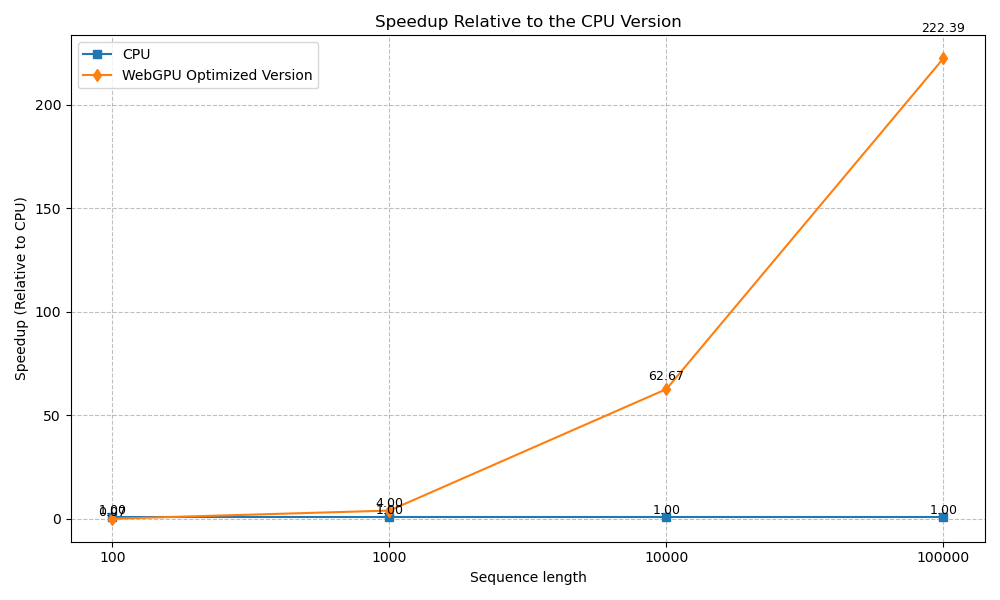
\includegraphics[width=1\linewidth]{uhd620.png}
  \caption{WebGPU-Optimized speed-up over CPU on Intel UHD 620}
  \label{fig:uhd620}
\end{figure}

\begin{figure}[h]
  \centering
  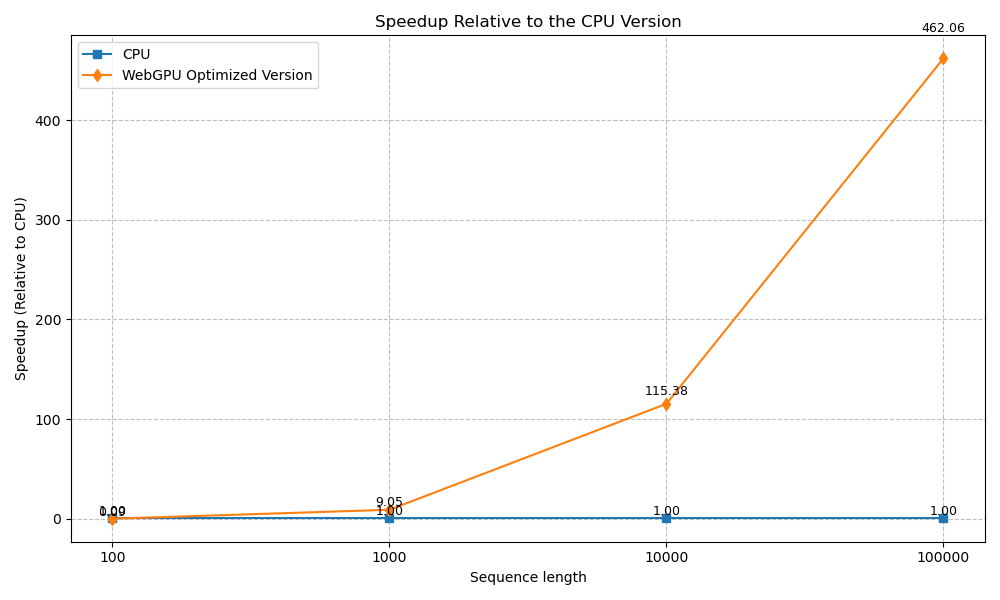
\includegraphics[width=1\linewidth]{m1.png}
  \caption{WebGPU-Optimized speed-up over CPU on Apple M1}
  \label{fig:m1}
\end{figure}

\begin{figure}[h]
  \centering
  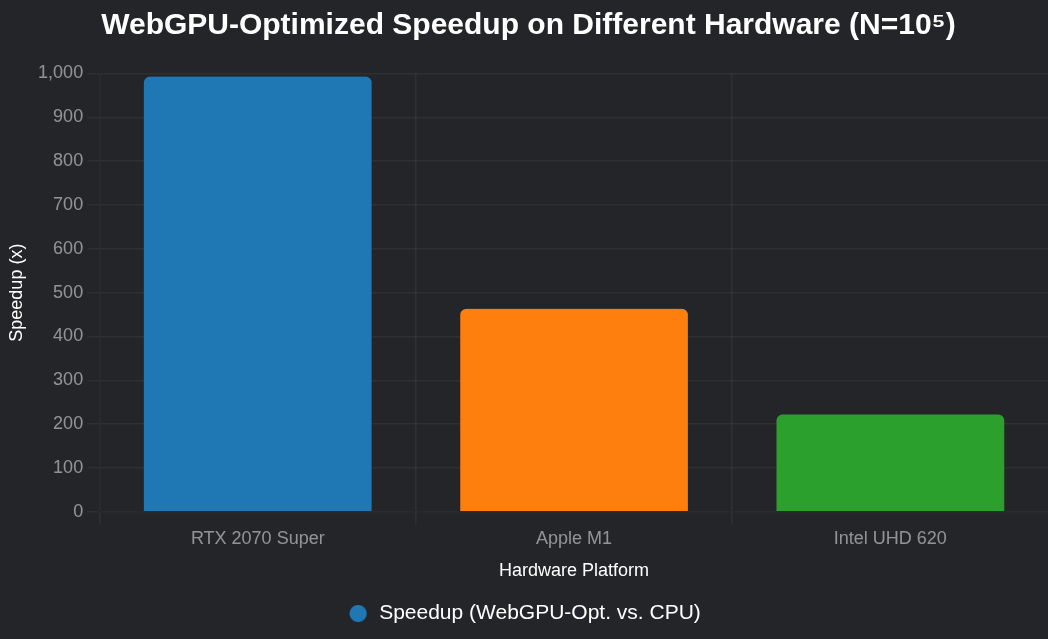
\includegraphics[width=1\linewidth]{比較不同硬體(RTX 2070 Super、M1、UHD 620)在 N=10⁵ 時的 WebGPU-Optimized 加速比.png}
  \caption{WebGPU-Optimized acceleration (CPU = 1.0) across three GPUs at $N=10^{5}$}
  \label{fig:cross-hw1}
\end{figure}
\clearpage

\section{Correctness Verification—Relative Log-Likelihood Error}
Using CUDA on the RTX~2070 Super as the reference\cite{NVIDIA2019-rtx2070,NVIDIA2023-cudaguide}, we define the relative error
\[
  \varepsilon(N)=
  \frac{\lvert LL_{\text{platform}}(N)-LL_{\text{CUDA}}(N)\rvert}
       {\lvert LL_{\text{CUDA}}(N)\rvert}\times100\,\%.
\]

\begin{table}[h]
  \centering
  \caption{Relative log-likelihood error (vs.\ CUDA, RTX 2070 Super)}
  \label{tab:likelihood_error}
  \setlength{\tabcolsep}{6pt}
  \renewcommand{\arraystretch}{1.9}
  \small
  \begin{tabularx}{\textwidth}{@{}X c c c c@{}}
    \toprule
    Platform / $N$      & $10^{2}$ & $10^{3}$ & $10^{4}$ & $10^{5}$ \\
    \midrule
    WGPU-Opt (RTX 2070 S)  & $2.5\times10^{-4}\,\%$ & $1.3\times10^{-5}\,\%$ & $2.2\times10^{-4}\,\%$ & $3.8\times10^{-4}\,\%$ \\
    WGPU-Opt (Apple M1)    & $2.8\times10^{-4}\,\%$ & $1.5\times10^{-5}\,\%$ & $2.2\times10^{-4}\,\%$ & $3.8\times10^{-4}\,\%$ \\
    WGPU-Opt (Intel UHD 620)& $2.5\times10^{-4}\,\%$ & $1.3\times10^{-5}\,\%$ & $2.2\times10^{-4}\,\%$ & $3.8\times10^{-4}\,\%$ \\
    \bottomrule
  \end{tabularx}
\end{table}
\newpage
\begin{figure}
    \centering
    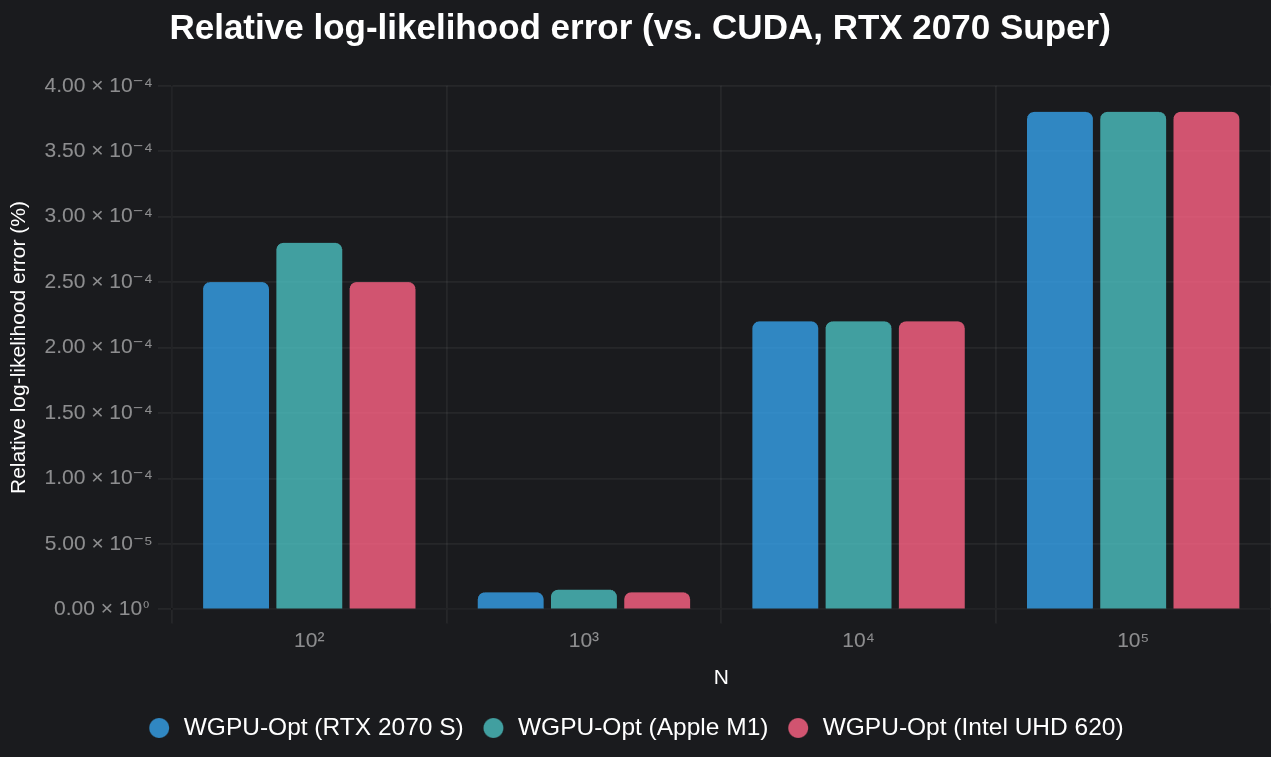
\includegraphics[width=1\linewidth]{Relative log-likelihood error.png}
    \caption{Bar chart displaying the relative log-likelihood error for \texttt{WGPU-Opt} on RTX~2070~S, Apple~M1, and Intel~UHD~620 versus CUDA on RTX~2070~Super, across $N$ values of $10^2$, $10^3$, $10^4$, and $10^5$.}
    \label{log-likelihood error}
\end{figure}

\section{Summary}
WebGPU-Optimized attains up to 84\% of CUDA performance on the RTX 2070 Super while retaining a three-order-of-magnitude advantage over single-threaded CPU execution\cite{Schmidt2024-gpuPairHMM}.  

On Apple M1 and Intel UHD 620, the same WGSL shader still delivers 4–463\,$\times$ acceleration, confirming that the two optimisations are portable and vendor-agnostic.  

Across all platforms, relative log-likelihood errors remain below $4\times10^{-4}\,\%$, demonstrating that high throughput does not come at the cost of numerical accuracy.  






\chapter{Discussion}

\section{Performance Analysis}
\subsection{RTX 2070 S: Performance Scaling and CUDA Gap}  
\begin{itemize}
  \item Versus single-threaded CPU, WebGPU-Optimized ranges from
        $1/0.165 \approx 6\times$ slower (at $N=10^{2}$) to nearly
        $1{,}000\times$ faster (at $N=10^{5}$); the larger the input,
        the greater the advantage.
  \item Compared with CUDA, WebGPU-Optimized starts at only
        $0.115$ of CUDA speed (i.e.\ $8.7\times$ slower) for
        $N=10^{2}$ owing to start-up and IPC overhead, but
        narrows the gap as $N$ increases, reaching
        $0.84$ of CUDA speed (84\%) at $N=10^{5}$.
\end{itemize}

At $N=10^{2}$, launch latency and inter-process communication dominate,
so WebGPU-Optimized is $8.7\times$ slower than CUDA.  
Dynamic Uniform Offsets amortise these costs as input length grows;
by $N=10^{5}$ the optimized browser-side kernel is within 19 % of CUDA,
with an absolute difference of just 0.53 s.

\subsection{Cross-GPU Bottlenecks}
Even on the RTX 2070 Super, our WebGPU-Optimized version still trails CUDA by up to 6 \%–19 \% in wall-clock time, while on Apple M1 and Intel UHD 620 it delivers tens- to hundreds-fold acceleration over single-threaded CPU code (Apple M1 \cite{Apple2020-m1}, Intel UHD 620 \cite{Intel2018-uhd620}). The residual gap therefore stems not from algorithmic flow but from the interaction between micro-architecture and API design. Two root causes emerge: SFU Throughput Bottleneck and resource-binding overhead.

\subsection{SFU Throughput Bottleneck}

On RTX~2070~S, both CUDA and WebGPU compile each
\texttt{log}/\texttt{exp} into \\ \texttt{MUFU.LOG/EX2}, so the
\emph{dependent latency} of a single transcendental
($\approx 12$ cycles on Turing) is identical.

The performance gap instead comes from \emph{issue bandwidth}:
within every SM sub-partition, all instructions—FP32 or SFU—must pass
through the \textbf{same warp issue slot}.
Moreover, the variable-latency SFU pipeline is only eight lanes wide,
so a 32-thread warp needs four cycles to be fully dispatched,
i.e.\ at most \textbf{one transcendental warp-issue every four cycles}.\cite{NVIDIA2023-cudaguide}

When three data-dependent \texttt{log}/\texttt{exp} appear back-to-back,
the warp must wait for the shared slot. CUDA kernels keep
$\geq 32$ resident warps, letting the scheduler interleave
independent warps to hide this stall.
In contrast, WebGPU shaders often have $<16$ active warps,
so SFU latency surfaces as a hard bottleneck.

Each DP cell in Pair-HMM invokes $\sim 12$ such operations;
for a 100\,000-base read, the kernel executes
$\mathcal{O}(10^{9})$ transcendentals, so the
\emph{throughput} limit of the SFU
becomes the dominant factor as $N$ grows.

\subsection{API Overhead: Pointer Rotation vs.\ BindGroup Reconstruction}
CUDA rotates three pointers (\texttt{prev}, \texttt{curr}, \texttt{new}) without allocation or validation\cite{NVIDIA2023-cudaguide}.  
WebGPU, however, must recreate a \texttt{BindGroup} whenever a binding changes because descriptors are immutable (W3C WebGPU \cite{W3C2024-webgpu}). Each \texttt{createBindGroup()} call traverses the V8 → Blink → Dawn → driver stack, incurring about $5$–$15$\,\textmu s. For $N=10^{5}$ the $2N$ anti-diagonals trigger roughly $200\,000$ such reconstructions, accumulating multiple seconds of delay.

Dynamic Uniform Offsets remove the need to rebind uniform data, yet the three mutable DP buffers still require $2N$ BindGroup creations. Resource-binding overhead therefore remains a key optimisation target for future WebGPU revisions that might allow in-place descriptor updates or bind-group recycling.




\subsection{Numerical Stability: Log-space \emph{versus} Scaling Coefficients}

\textit{(Scaling has not yet been implemented in the current prototype; this section evaluates its feasibility.)}

The present WebGPU kernel uses the conventional \emph{log-space} formulation to avoid underflow on long read–haplotype pairs \cite{Durbin1998}.  
While mathematically robust, each dynamic-programming (DP) cell requires one \texttt{exp} and one \texttt{log}, hitting WebGPU’s software-emulated SFU pipeline twice per update \cite{NVIDIA2023-cudaguide} .

\vspace{0.4em}
\noindent\textbf{Scaling as an alternative.}\;
Instead of converting the entire recurrence to log space, one can remain in probability space and renormalise after each column:

With values now confined to $[0,1]$, the inner loop no longer calls \texttt{log}/\texttt{exp}.  
After the DP completes, the stored $c_{t}$ values are converted back into the overall log-likelihood by summing their logarithms and applying a minus sign.  
This keeps numerical stability while sharply reducing SFU traffic and easing register and memory pressure.

\paragraph{Potential benefits}
\begin{itemize}
  \item \emph{Reduced SFU usage}—all inner-loop work becomes plain \texttt{f32} multiply–adds; transcendental functions are invoked only once at the end.
  \item \emph{Lower register pressure}—no need to keep log-transformed values alive across iterations.
  \item \emph{Vector-friendly data}—probabilities remain in $[0,1]$, facilitating SIMD execution and shared-memory tiling.
\end{itemize}

\paragraph{Trade-offs and implementation notes}
\begin{enumerate}
  \item Each column now requires a workgroup-level reduction to compute $c_{t}$.  
        Although this can be implemented with barrier-synchronised tree sums, it introduces extra global synchronisation absent from the log-space variant.
  \item All $c_{t}$ (or $\log c_{t}$) values must be stored for the final likelihood recovery, adding an $O(T)$ buffer that grows with read length.
  \item Scaling is numerically safe only when the column sum is well conditioned; highly skewed emissions may still require occasional re-normalisation safeguards.
\end{enumerate}

\paragraph{Outlook}
Given the sizeable SFU share in the current profile, the scaling scheme could shift the hotspot entirely to ALU pipelines and fit well with future subgroup-shuffle intrinsics.  
A full conversion, however, would require revisiting the bind-group layout and workgroup granularity to hide the extra reduction cost.  
Quantitative evaluation is left for future work once subgroup support and finer-grained shader timers become available.

\section{Numerical Stability and Error Analysis}
Across all three GPU architectures and all sequence lengths, the relative log-likelihood error stays below $3.8\times10^{-4}\,\%$.
\begin{itemize}
  \item \textbf{Sequence-length independence.} From $N=10^{2}$ to $10^{5}$, the error varies only between $1.3\times10^{-5}\,\%$ and $3.8\times10^{-4}\,\%$, indicating that floating-point round-off does not amplify with longer reads.
  \item \textbf{Hardware consistency.} NVIDIA, Apple, and Intel show near-identical error curves, implying that differences in SPIR-V / Metal translation and driver-level \texttt{f32} arithmetic (\texttt{fma}, \texttt{log}, \texttt{exp}) have negligible impact on the final likelihood.
  \item \textbf{Consistency with theory.} IEEE-754 single precision has a machine-epsilon of roughly $1.19\times10^{-7}$. After $10^{5}$ iterations, the worst observed relative error ($3.8\times10^{-6}$ as a fraction) remains within the same order of magnitude, confirming numerical stability.
\end{itemize}

\paragraph{Origin of the residual error.}
Although the algorithm is identical, moving from CUDA to WebGPU introduces several hardware- and driver-level differences that accumulate tiny floating-point deviations:
\begin{itemize}
  \item \textbf{FMA fusion policy.} CUDA guarantees that every \texttt{a*b+c} is fused into a single FMA (one rounding), whereas WebGPU shaders may emit a separate multiply and add, causing an extra rounding step.
  \item \textbf{Polynomial approximations for \texttt{log}/\texttt{exp}.} CUDA’s \texttt{libdevice} and each WebGPU driver use different coefficients, typically differing by up to $\pm$3–4 ULP, which translates into $\approx10^{-6}$ fractional error after thousands of calls.
  \item \textbf{Flush-to-Zero (FTZ) handling.} Mobile or integrated GPUs often enable FTZ by default in WebGPU, zeroing sub-normal values that CUDA still represents exactly, slightly perturbing sums of very small probabilities.
  \item \textbf{Compiler reassociation.} During WGSL $\rightarrow$ SPIR-V/Metal optimization, common-subexpression elimination and reassociation can legally reorder floating-point additions, changing the rounding path while remaining IEEE-754 compliant.
\end{itemize}

\paragraph{Implications for variant calling.}
Production pipelines such as GATK typically tolerate log-likelihood errors in the $10^{-2}$–$10^{-3}$ range \cite{McKenna2010}. Our WebGPU implementation is two orders of magnitude tighter, ensuring that browser-based execution maintains scientific correctness for downstream variant calling.





\section{Lessons from \textit{gpuPairHMM}}
Recent work by Schmidt \emph{et~al}. on \textit{gpuPairHMM} shows that a wavefront-based, register-resident kernel combined with warp-shuffle intrinsics can reach up to $2.6$ TCUPS (trillions of cell updates per second) on an NVIDIA L40S, outperforming prior GPU, CPU, and FPGA implementations by more than an order of magnitude \cite{Schmidt2024-gpuPairHMM}. Three design decisions are particularly instructive for WebGPU:

\begin{itemize}
  \item \textbf{Sub-warp diagonal tiling \& warp shuffle.}  
        Each sub-warp owns a diagonal tile and exchanges boundary values through \texttt{\_\_shfl\_sync}.  
        Although WGSL currently lacks explicit shuffle intrinsics, the same register-tile principle can be emulated with workgroup memory plus \\ \texttt{workgroupBarrier()} once subgroup operations become standard.
  \item \textbf{Emission memoisation \& length-aware kernels.}  
        \textit{gpuPairHMM} caches only five distinct emission probabilities and specialises kernels by (readLen, hapLen) buckets, sharply reducing divergence and register pressure.  
        WebGPU can mirror this behaviour by maintaining multiple pre-compiled pipelines and indexing a compact \texttt{storage} buffer that stores the five emission scores.
  \item \textbf{Host–device overlap.}  
        The authors hide PCIe latency with multiple CUDA streams.  
        While browsers cannot issue true DMA, the pattern can be approximated by double-buffered \texttt{queue.writeBuffer()} / \texttt{queue.submit()} pairs.  
        Such overlap will be critical for sustaining throughput once our implementation moves from integrated GPUs to discrete adapters.
\end{itemize}

Adopting these tactics should further improve WebGPU performance without altering the underlying Pair-HMM algorithm.

\section{Cross-Hardware Performance}

\subsection{Apple M1: Pros and Cons of a Unified-Memory Architecture (UMA)}
Apple’s M1 employs a UMA design that shares 8 GB of LPDDR4X between CPU and GPU, eliminating discrete memory transfers \cite{Apple2020-m1}.  
For moderate $N$ values, \texttt{copyBufferToBuffer()} degrades to a pointer-offset adjustment rather than true DMA, reducing WebGPU start-up latency relative to discrete GPUs.

At large $N$, however, CPU–GPU bandwidth contention emerges, and the M1 remains about $2.2\times$ slower than the RTX 2070 Super.  
Nevertheless, WebGPU-Optimized delivers a $463\times$ speed-up over single-threaded CPU execution, demonstrating that Dynamic Uniform Offsets effectively hide latency even under unified memory.

\subsection{Intel UHD 620: Driver Maturity and Scheduling Strategy}
The UHD 620 lacks hardware SFUs and offers only 24 execution units, making \texttt{log}/\texttt{exp} workloads expensive \cite{Intel2018-uhd620}.  
The Chrome–Dawn–DX12 stack serialises command submission via a submit-fence pattern, leaving the CPU idle for small $N$.

Its 768 KB L3 cache is easily thrashed when multiple storage buffers interleave, causing frequent L2 misses.  
Despite these constraints, our optimisations still achieve a $222\times$ speed-up at $N = 100\,000$.

These results confirm that the proposed WebGPU optimisations are vendor-agnostic and can improve performance even on low-end integrated GPUs, underscoring WebGPU’s potential as a truly cross-platform acceleration framework.





\chapter{Future Work}

This study demonstrates that two \textbf{WebGPU-oriented optimizations} single—\texttt{CommandBuffer} batch submission and Dynamic Uniform Offsets—can reduce browser-side runtime for the \emph{Pair-HMM Forward} algorithm to within a constant factor of native CUDA. Although this performance suffices for online demonstrations and interactive teaching, larger clinical pipelines and cloud back-ends demand further gains. We therefore outline three promising research directions—API, algorithmic, and ecosystem levels—together with concrete implementation paths and anticipated challenges.

%------------------------------------------------
\section{Closing the Double-Precision Gap}

Double-precision (\textbf{FP64}) support is critical to many scientific workloads. WebGPU currently guarantees only \textbf{FP32} operations even on hardware with native FP64 units—e.g.\ NVIDIA RTX 40 series or Apple M2 Max—because WGSL lacks an \texttt{f64} type \cite{W3C2024-webgpu,NVIDIA2023-cudaguide,Apple2023-m2max}. For \emph{Pair-HMM}, single precision typically keeps relative error below $10^{-5}$, but very long reads risk underflow.

\subsection*{Mixed-Precision Techniques}

\paragraph{Implementation path}
\begin{itemize}
  \item Isolate numerically sensitive stages such as log-likelihood accumulation.
  \item Emulate FP64 by splitting a 64-bit value into two \textbf{FP32} parts, or by modular WGSL routines for double-precision arithmetic.
  \item Retain \textbf{FP32} elsewhere to preserve throughput.
\end{itemize}

\paragraph{Challenges}
\begin{itemize}
  \item Software FP64 increases ALU pressure, potentially offsetting WebGPU gains.
  \item Accuracy varies across GPUs due to differing \textbf{FP32} semantics, requiring extensive regression tests.
  \item Approximation error may accumulate over very long sequences and needs validation against ground-truth data.
\end{itemize}

%------------------------------------------------
\section{Hybrid Acceleration with WASM+SIMD and WebGPU}

WebGPU excels at high throughput, but its fixed API overhead can dominate for short reads. A hybrid model that combines \textbf{WebAssembly (WASM)} plus 128-bit \textbf{SIMD} for small inputs with WebGPU for large inputs can bridge this gap \cite{MDN2023-simd}.

\subsection{Short sequences ($N < 512$)}

\paragraph{Implementation path}
\begin{itemize}
  \item Write a SIMDintrinsic-optimized WASM module in Rust / C++ for the DP kernel.
  \item Add a JavaScript dispatcher that selects WASM+SIMD for short inputs and WebGPU for longer ones, avoiding GPU cold-start latency.
  \item Cache the compiled WASM to amortize instantiation cost.
\end{itemize}

\paragraph{Challenges}
\begin{itemize}
  \item Initial WASM compilation may dominate tiny inputs; caching strategies are essential.
  \item SIMD ISA differs across x86 and ARM, requiring portable intrinsics or multiple builds.
  \item Hybrid debugging and profiling is more complex than single-backend workflows.
\end{itemize}

\subsection{Long sequences}

\paragraph{Implementation path}
\begin{itemize}
  \item Batch thousands of reads per dispatch to maximize GPU occupancy.
  \item Align input buffers with the WebGPU parallelism model.
  \item Optimize command-buffer submission to reduce CPU–GPU synchronizations.
\end{itemize}

\paragraph{Challenges}
\begin{itemize}
  \item On non-UMA systems, CPU–GPU transfers remain a bottleneck; buffer packing and compression may help.
  \item Dispatch sizes must balance occupancy against memory limits.
\end{itemize}





\section{Distributed Execution Across Edge and Cloud}

Browser-resident WebGPU suffices for moderate datasets but not for clinical workloads spanning millions of bases\cite{W3C2024-webgpu,MDN2025-webgpuapi}.  
A distributed framework can reconcile local interactivity with large-scale throughput\cite{Krampis2012,Stone2010-opencl}.

\paragraph{Implementation path}
\begin{itemize}
  \item Build a JavaScript scheduler that profiles the local adapter via \\ \texttt{navigator.gpu.adapter}\cite{MDN2025-webgpuapi}.
  \item Execute lightweight jobs locally; off-load heavy tasks to cloud nodes over WebRTC / WebSocket\cite{W3C2024-webgpu}.
  \item Run WebGPU-enabled containers in the cloud and stream partial results back incrementally\cite{Krampis2012}.
\end{itemize}

\paragraph{Challenges}
\begin{itemize}
  \item Large transfers demand compression and incremental protocols to mask latency\cite{Stone2010-opencl}.
  \item Ensuring privacy and standardizing WebGPU drivers in the cloud add operational overhead\cite{W3C2024-webgpu}.
  \item Scheduler logic must predict load and latency, complicating design\cite{Krampis2012}.
\end{itemize}


\section*{Conclusion}

The three avenues—mixed precision for FP64, WASM+SIMD/WebGPU hybridity, and edge–cloud distribution—tackle precision, latency, and scale, respectively. Pursuing them can elevate WebGPU-accelerated genomic analysis from a teaching prototype to a production-ready, high-precision, and scalable solution without changing the underlying \emph{Pair-HMM} algorithm.







\chapter{Conclusion}

This work presents the first complete browser-side implementation of the Pair-HMM Forward algorithm using WebGPU, filling a gap left by earlier CUDA-centric studies \cite{Banerjee2017,Schmidt2024-gpuPairHMM}.  
We systematically evaluate four implementations—C++, CUDA, WebGPU-Baseline, and WebGPU-Optimized—across three heterogeneous GPUs (RTX 2070 Super, Apple M1, and Intel UHD 620), analysing both performance and numerical correctness.

%------------------------------------------------
\section{Core Contributions}

\begin{enumerate}
  \item \emph{Two complementary browser-side optimizations.}\\
        The proposed techniques—single-\texttt{CommandBuffer} batch submission and Dynamic Uniform Offsets—\emph{jointly reduce} CPU–GPU round-trips \emph{and} minimise BindGroup reconstruction overhead.  
        For a sequence length of $N = 10^{5}$ on the RTX 2070 Super, these optimizations cut run time from $466$ s (Baseline) to $3.3$ s, achieving $84\,\%$ of CUDA performance.

  \item \emph{Cross-device validation.}\\
        The same WGSL shader delivers $4$–$222\times$ speed-ups on Intel UHD 620 \cite{Intel2018-uhd620} and $9$–$463\times$ on Apple M1 \cite{Apple2020-m1}, confirming that the optimizations are vendor-agnostic—any browser with WebGPU support can enable GPU acceleration without native-driver installation.

  \item \emph{A reproducible workflow for porting bioinformatics DP algorithms to the web.}\\
        We provide WGSL kernels and tuning strategies that address known WebGPU bottlenecks, creating a template for porting wavefront-based algorithms such as Smith–Waterman and Needleman–Wunsch to the browser \cite{Ghosh2018}.
\end{enumerate}

%------------------------------------------------
\section{Academic and Industrial Impact}

WebGPU is not merely a drop-in replacement for installing CUDA SDKs or provisioning cloud GPUs; it enables real-time computation inside the browser sandbox, with zero driver installation and local data residency \cite{W3C2024-webgpu}.  
Researchers can now run Pair-HMM likelihood estimation on laptops and integrated-GPU (iGPU) systems while retaining full data control, thereby lowering the barrier for classroom use, clinical front-ends, and interactive open-science platforms \cite{Chrome2024-blog}.

In summary, the demonstrated paradigm—driver-free, cross-hardware, and fully on-device—charts a practical path toward browser-native scientific GPU computing.  
As browser APIs and GPU hardware continue to evolve, we anticipate that many genomics applications will become fully web-executable within the next three to five years, further democratising high-performance bioinformatics and accelerating digital transformation in biomedical research.




\newpage
\AddToContents{Bibliography}
\printbibliography[
  heading=bibintoc,
  title={Reference}
]
\end{document}